\documentclass{article}
\usepackage{a4wide}
\usepackage[utf8]{inputenc}
\usepackage[T1]{fontenc} 
\usepackage{fancyhdr} 
\usepackage{graphicx}
\usepackage{lastpage}
\usepackage{enumerate}
\usepackage{amssymb}
\usepackage{amsmath} 
\usepackage{algorithm}
\usepackage{tikz} 
\usepackage{listings}
\usepackage[noend]{algpseudocode}
\usetikzlibrary{automata, arrows}
\usepackage{subcaption}
\usepackage{hyperref}
\usepackage{booktabs}

\makeatletter
\def\BState{\State\hskip-\ALG@thistlm}
\makeatother



\lhead{
\includegraphics[width=4.6cm]{uni.png}\\ \course\\ \semester\\Segmentation of Femurs \homeworkNumber}
\rhead{\university\\ \authorname\\\authoremail\\Page \thepage\ of \pageref{LastPage}}

\usepackage[headheight=68pt]{geometry}
\pagestyle{fancy}

%% Custom command
\newcommand{\authorname}{Giorgi Grigalashvili, Fabricio Arend Torres}
\newcommand{\authoremail}{\{g.grigalashvili, fabricio.arendtorres\} @ stud.unibas.ch}
\newcommand{\semester}{Spring Semester 2017}
\newcommand{\course}{Probabilistic Shape Modelling}
\newcommand{\homeworkNumber}{}

\newcommand{\university}{University of Basel}
\newcommand{\department}{Department of Mathematics and Computer Science}
\newcommand{\address}{Spiegelgasse 1, 4051 Basel, Switzerland}
\newcommand{\website}{dmi.unibas.ch / informatik.unibas.ch}

%% Custom commands

\def\underline#1{\underline{\underline{#1}}}

\begin{document}
	\author{Giorgi Grigalashvili, Fabricio Arend Torres}
		\title{Project 2:\\ Femur Segmentation from CT Scans}
	\maketitle
	\begin{abstract}
		In this second project, we implemented a sampling procedure that allows us to automatically segment femurs from CT scans by using a provided active shape model.
		The basic idea relies on the combination of a pixel intensity model and a statistical shape model.
		Through MCMC sampling it is possible to estimate an optimal fit in terms of the posterior probability of the model given the CT scan in form of a '.nii' image.
	\end{abstract}
	

	\section{Introduction}
	Automated image segmentation in the medical field poses a difficult problem which could significantly improve many processes.
	The difficulty arises due to partial volume effects, artifacts in the image and general noise.
	The aim of the project is the segmentation of 5 femurs, for each of which a CT scan image is provided. 
		
	The approach presented in this paper relies on an active shape model(ASM) for femurs, which is a combination of a statistical shape model and an intensity model.
	The Shape Model provides a probability distribution over femur shapes, which was presumably learned from observed data.
	The intensity model models the intensities at areas around given profile points of the shape model.	


	\section{Method}
	Our aim is finding a femur shape defined by the parameter set $\theta$ which explains the image intensities observed in the CT as good as possible while still considering realistic and likely femur shapes.
	More formally we search for the following maximum a posteriori estimation:
	\begin{equation}
	\theta^* = \arg\max_\theta \frac{p(\theta) P(I_T | \theta)}{\int p(\theta) p(I_T | \theta) \delta\theta}
	\end{equation}	
	So the likelihood of the observed image as well as the prior probability of the parameters that define a shape are necessary.
	
	The used ASM models the image intensities as normal distributions for specific profile points, which lie orthogonal to the shapes.
	In the segmentation procedure we can use this for evaluating the likelihood for observing intensities at the position of the profile points for a specific shape instance.
	The mean intensities of the provided ASM are visualized in \autoref{1.1}.
	With this we have:
	\begin{equation}
	p(I_T | \theta) = \mathcal{N}(\mu_i, \Sigma_i) 
	\end{equation}
	where $\theta$ is a possible set of parameters that defines an instance of the shape model.
	By assuming that the noise at the different profile points is independent and identically distributed, we can calculate the total likelihood of an image by taking the product of the likelihoods.	
	\begin{equation}
	p(I_T|\theta) = \prod_{i} \mathcal{N}(\mu_i, \Sigma_i)
	\end{equation}
	
	The prior probability $p(\theta)$ is provided by the statistical shape model of the ASM, which was learned from 25 femurs.
	While just the prior and the likelihood do not suffice for defining the posterior probability, we can use those for Metropolis Hastings algorithm, where the posterior probability is approximated through repeated sampling of parameters.
	
	New proposals are sampled under use of a Proposal Generator:
	\begin{equation}
	Q(\theta' | \theta) = N(\theta'|\theta, \Sigma_\theta)
	\end{equation}
	Each time a new sample $\theta'$ is generated, it is accepted with the probability 
	\begin{equation}
	min \{ \frac{P(\theta' | D ) Q(\theta|\theta')}{P(\theta|D) | Q(\theta'|\theta)}, 1\}
	\end{equation}
	Under certain conditions, this sampling procedure is guaranteed to converge to the posterior probability.
	
	We made use of two different but similar proposal mechanisms:
	\begin{enumerate}
		\item A random walk of $\theta$, where all parameters in the set $\theta$ are updated at once with: 
		$$\theta_{proposed} = \theta_{old} + d \quad d \sim \mathcal{N}(0,\sigma I)$$
		\item A random walk of $\theta$, where only one individual parameter $theta^{(i)}$ is updated with: 
		$$\theta_{proposed}^{(i)} = \theta_{old}^{(i)} + d \quad d \sim \mathcal{N}(0,\sigma)$$
	\end{enumerate}
	
	Multiple of such proposals with different $\sigma$ (or different target parameters for the 2nd method) have then been combined into a big mixed proposal generator.
	The individual values and sample probabilities are displayed in the following table.
	It should be noted, that the probabilities of each 'update type' sum to one.
	The final mixture proposal first selects one of the two methods with the probability $0.5$ and then a specific version of that with the following probabilities:
	\begin{figure}
		\centering
		%\begin{subfigure}{.5\textwidth}
			\centering
			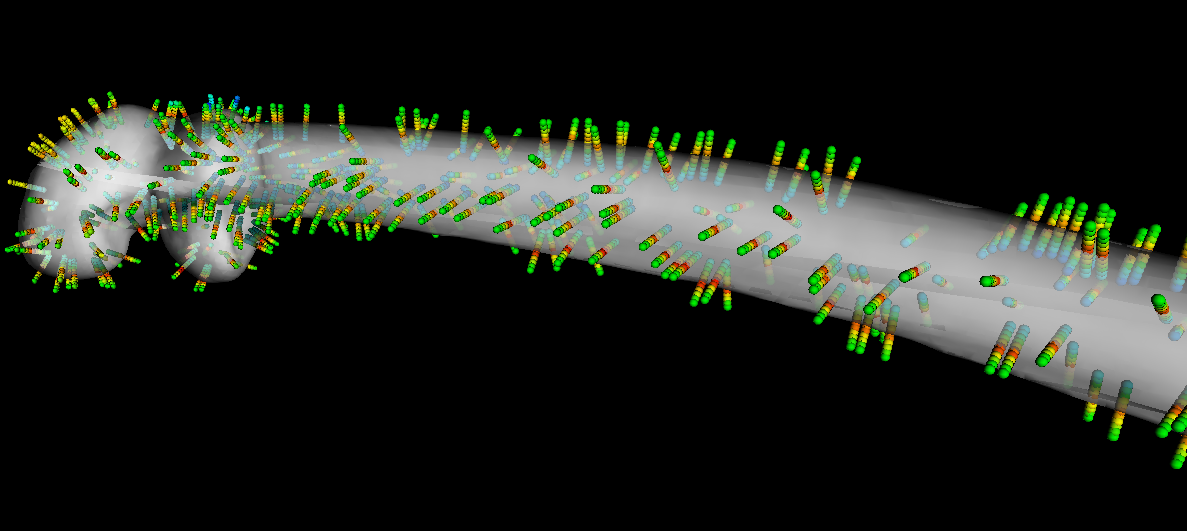
\includegraphics[width=0.8\textwidth]{images/mean_pixelintensities.png}
			\caption{Mean Intensities and mean shape of the ASM}
			\label{1.1}
		%\end{subfigure
	\end{figure}	
	As we are only interested in the MAP shape, we did not bother specifying a burn-in phase before drawing samples.

	\begin{center}
		\begin{tabular}{l l l l l}
			\toprule
			update type & $\sigma$ & Probability \\
			\midrule
			Batch Random Walk $N(0, \sigma I)$&  0.001 & 	0.2  	\\
			Batch Random Walk $N(0, \sigma I)$& 0.01 & 	0.4 	\\
			Batch Random Walk $N(0, \Sigma I)$& 0.05 &	0.2		\\
			Batch Random Walk $N(0, \Sigma I)$& 0.2&		0.2		\\
			Single Parameter Random Walk $N(0,\sigma)$ & 0.1& $\frac{1}{rank(ShapeModel)}$
		\end{tabular}
	\end{center}
	\section{Results \& Discussions}
		The main problem that we faced was the very low acceptance rate with the initial update scheme (only batch updates, ~100 accepted for 10000 drawn samples).
		Our approach for fixing this was based on using smaller updates for the proposals as well including updates of individual parameters.
		Although that increased the sample rate a little bit, the acceptance rate is still rather low with $\sim 5\%$ (~250 accepted for 5000 drawn samples).
		
		Another problem that we faced was an error occurring at the likelihood evaluation of the CT image \textit{10.nii}. We assume this was caused by instances of the femur shape that were out of the CT images range (see \autoref{2.2}). As such there were no intensities that could be evaluated. 
		Furthermore this image differs from the other ones, as it also contains another foot of the scanned person (see \autoref{2.1}), but this did not cause any complications.
	
		Besides that, the segmentation seems to be successful, as far as we can judge.
		When looking at the fitted shape in context of the CT image, it mostly coincides with intuitive understanding of where the femurs should be.
		The test segmentations are also very similar to the provided groundtruths.
		The few differences could be either be because the sampling did not run long enough or because the used statistical shape model can not model some variations (as it was only generated by 25 femurs).
		In figure \autoref{3d} and \autoref{slice} the segmented femurs a visualized in context of the CT image.
		
\begin{figure}
	\centering
	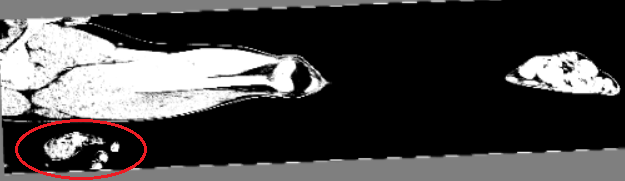
\includegraphics[width=0.7\textwidth]{images/CT_10_foot.png}
	\caption{Artifacts in the CT scan: another foot}
	\label{2.1}
\end{figure}		
\begin{figure}
	\centering
	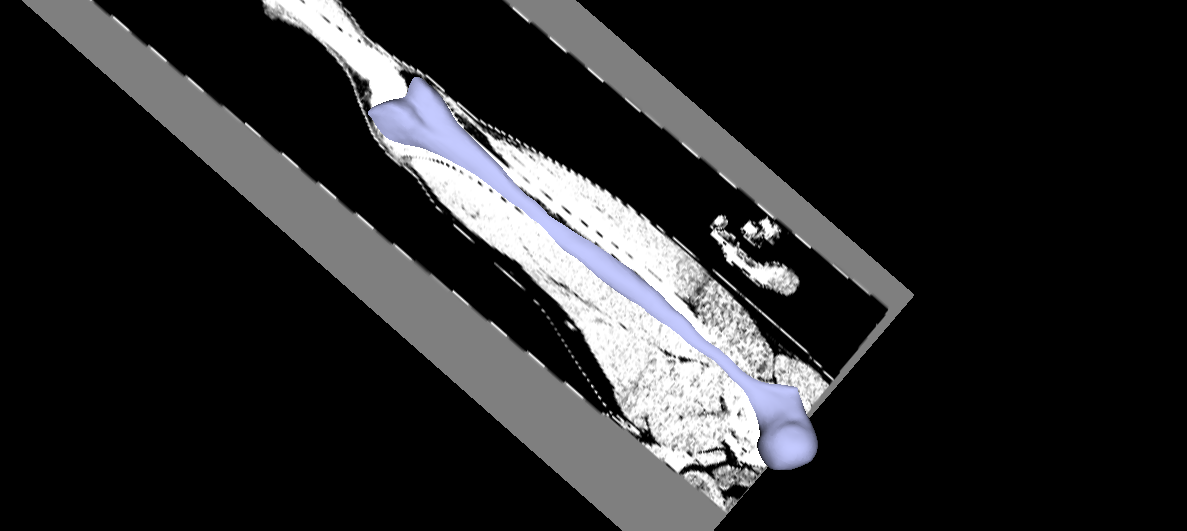
\includegraphics[width=0.7\textwidth]{images/segmentation_10_outofrange.png}
	\caption{Possible Variations may be out of range of the CT image}
	\label{2.2}
\end{figure}
\begin{figure}
	\centering
	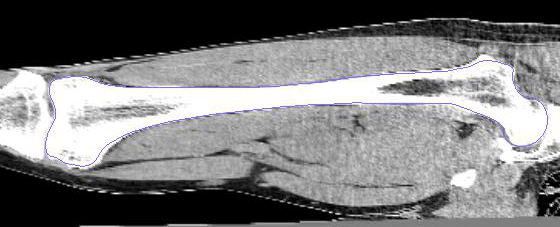
\includegraphics[width=0.7\textwidth]{images/border_segmentation1.png}
	\caption{Slice view of the segmented femur}
	\label{slice}
\end{figure}
\begin{figure}
	\centering
	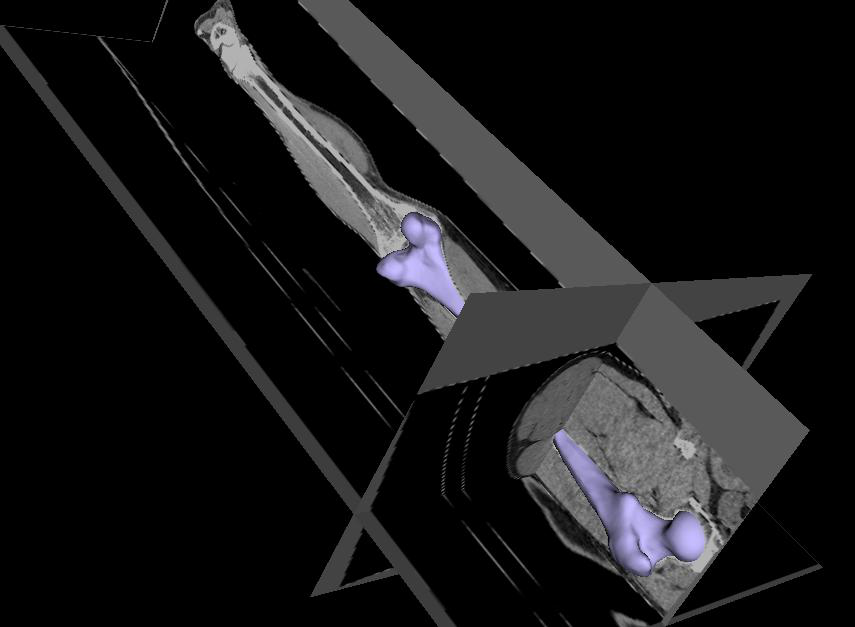
\includegraphics[width=0.6\textwidth]{images/3dSegmentation.png}
	\caption{3D view of the segmented femur}
	\label{3d}
\end{figure}

\end{document}